% !TeX spellcheck = cs_CZ
%{\tikzset{external/prefix={tikz/FYZI/}}
% \tikzset{external/figure name/.add={ch53_}{}}
%---------------------------------------------------------------------------------------------------
% file kinematika.tex
%---------------------------------------------------------------------------------------------------
\setchaptertoc
\chapter{Kinematika částice}

  Nejjednodušší fyzikální soustava je jeden hmotný bod, který se pohybuje v prostoru a čase. Pojem
  hmotný bod je ovšem abstrakce, model, kterým nahrazujeme reálnou částici. Vyjadřujeme jím, že
  odhlížíme od tvaru a rozměru částice, považujeme ji za bodovou, a kromě její geometrické polohy v
  daném okamžiku jí připisujeme pouze jedinou fyzikální vlastnost, hmotnost. V tomto smyslu budeme
  v mechanice často místo hmotného bodu hovořit prostě o částici.
  %----------------- Kinematický popis pohybu částice --------------------------------------------- 
  \section{Kinematický popis pohybu částice}
    V kinematice se zajímáme pouze o průběh pohybu částice v prostoru a čase a nepátráme po
    příčinách tohoto pohybu a jeho změn. Předpokládáme, že částice se pohybuje po spojité křivce,
    trajektorii, a snažíme se určit jednak tvar této trajektorie a zákon pohybu po ní, tj. polohu
    částice na trajektorii v závislosti na čase\footnote{Představa o pohybu částice po trajektorii
    jako po spojité křivce vyplývá z naší smyslové zkušenosti. Ukazuje se, že v mikrosvětě tato
    představa neodpovídá skutečnosti a pojem trajektorie tam ztrácí smysl. Částice se v mikrosvětě
    pohybuje podle zákonu kvantové mechaniky a v daném okamžiku není možné současné přesně stanovit
    její polohu a rychlost}. Spojitá křivka má v každém bodě tečnu a můžeme zavést pojem okamžité
    rychlosti částice mířící ve směru této tečny.
  
    \begin{figure}[ht!]
      \centering
      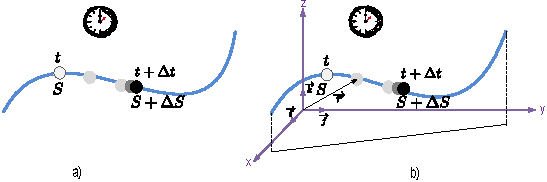
\includegraphics[width=\linewidth]{fyz_fig227.pdf}
      \caption{Příklad trajektorie částice a zavedení kartézské soustavy souřadnic}
      \label{fyz:fig227}
    \end{figure}
  
    Předpokládejme nejprve, že trajektorie částice je zadána. Pak můžeme od zvoleného bodu na
    trajektorii a zvoleného okamžiku měřit dráhu částice $s(t)$, tedy délku křivky, kterou částice
    za určitou dobu prošla (obr. \ref{fyz:fig227}). V okamžiku $t$ je částice v bodě daném
    prošlou dráhou $s$, v okamžiku $t + \Delta t$ v bodě $s + \Delta s$. Dráha $s$ tu vlastně
    představuje parametr udávající polohu bodu na křivce; tímto způsobem popisujeme například pohyb
    automobilu na dálnici a udáváme na kterém je právě kilometru.
  
    Přitom můžeme zavést \textbf{střední rychlost částice} v intervalu $\Delta t$
    \begin{equation}\label{mech:eq_stredni_rychlost}
      \langle v\rangle=\frac{\Delta s}{\Delta t},
    \end{equation}
    \textbf{okamžitou rychlost částice} v okamžiku $t$
    \begin{equation}\label{mech:eq_okamzita_rychlost}
      v(t)=\lim_{\Delta t\rightarrow0}\frac{\Delta s}{\Delta t}=\frac{ds}{dt}=\dot{s}
    \end{equation}
    a \textbf{okamžité zrychlení}
    \begin{equation}\label{mech:eq_okamzite_zrychleni}
      a(t)=\lim_{\Delta t\rightarrow0}\frac{\Delta v}{\Delta t}
          =\frac{dv}{dt}=\lim_{\Delta t\rightarrow0}\frac{d^2s}{dt^2}=\dot{v}=\ddot{s}
    \end{equation}
    Takto zavedené rychlost a zrychlení jsou skalární funkce času a udávají pouze jak se mění dráha
    a rychlost při pohybu po zadané trajektorii, ve směru tečny k této trajektorii.
  
    Obecně však musíme udat polohu částice v prostoru vzhledem k nějaké vztažné soustavě. Tato
    soustava, například kartézská, je spojena s nějakým tuhým tělesem a doplněna hodinami
    umístěnými   například v počátku. V místnosti mohou jako kartézské osy sloužit průsečnice stěn
    a podlahy. Potom udáváme tři kartézské souřadnice částice jako funkce času:
    \begin{equation}\label{mech:eq_xyz}
      x=x(t),\quad y=y(t),\quad z=z(t)
    \end{equation}
    Soustava tří rovnic (rov. \ref{mech:eq_xyz}) představuje parametrické vyjádření tvaru
    trajektorie. Rovnici trajektorie v kartézských souřadnicích dostaneme, vyloučíme-li z rov.
    \ref{mech:eq_xyz} čas. Parametrem pohybu může být ovšem i dráha:
    \begin{equation}\label{mech:eq_draha}
      x = x(s),\quad y = y(s),\quad z = z(s).
    \end{equation}
    Přitom $s = s[x(t), y(t), z(t)]$ vystupuje jako složená funkce času. Výše zavedená skalární
    rychlost bude
  
    %-------------------------- Základní pohyby a jejich skládání-----------------------------------
    \subsection{Základní pohyby a jejich skládání}
      Uvedeme nyní některé základní typy pohybu částice.
      \subsubsection{Pohyb přímočarý}
          Nechť přímočarý pohyb probíhá podél osy x s počátečními podmínkami $x = x_0,v_x =
          \dot{x}=v_{0_x}$ při $t = t_0$. Pak rozlišujeme
          \begin{itemize}
            \item \emph{Pohyb rovnoměrný} s konstantní rychlostí $v_{0_x}$ a nulovým zrychlením
                  $a_x=0$. Integrací a použitím počátečních podmínek dostáváme zákon pohybu:
                  \begin{equation}\label{mech:eq_primocar_rovnomer}
                    x=x_0+v_{0_x}(t-t_0)
                  \end{equation}
            \item \emph{Pohyb rovnoměrně zrychlený} s konstantním zrychlením $a_{0_x}$ kladným nebo
                  záporným. Integrací a použitím počátečních podmínek dostáváme zákon ry\-chlo\-sti a
                  zákon pohybu:
                  \begin{align}
                    v &= v_0x+a_0x(t-t_0), \\
                    x &= x_0+v_{0_x}(t-t_0)+\frac{1}{2}a_{0_x}(t-t_0)^2 \label{mech:eq_const_acc}.
                  \end{align}
                  Je-li při $t = 0 x = 0, v = 0$ dostaneme známé vztahy $$v=a_{0_x}t,\quad
                  x=\frac{1}{2}a_{0_x}t$$
            \item \emph{Pohyb nerovnoměrný} se zrychlením obecně závislým na čase $a(t)$. Pak
                  do\-sta\-ne\-me zákon rychlosti a zákon pohybu integrováním
                  \begin{align}
                    v &= v_{0_x}+\int_{t_0}^{t}{a(t)dt} \\
                    x &= x_0+v_{0_x}(t-t_0)+\int_{t_0}^{t}{v(t)dt}
                  \end{align}
          \end{itemize}
      \subsubsection{Pohyb kruhový}
      \subsubsection{Pohyb harmonický}
        Pohyb harmonický dostaneme jako projekci rovnoměrného kruhového pohybu kolem počátku do
        jedné z kartézských os. Například v ose $y$ pak máme
        \begin{equation}\label{mech:eq_p_harmon}
          y(t)=A\sin(\omega t+\varphi_0)
        \end{equation}
        kde 
        \begin{labeling}{$\omega t+\varphi_0$}
          \setlength{\itemindent}{2cm}
          \item[\(y\)]                     \(\ldots\) \emph{výchylka (elongace)}, 
          \item[\(A\)]                     \(\ldots\) \emph{amplituda}, 
          \item[\(\omega\)]                \(\ldots\) \emph{úhlová rychlost} $[rad\cdot s^{-1}]$,
          \item[\(T=\frac{2\pi}{\omega}\)] \(\ldots\) \emph{perioda} $[s]$, 
          \item[\(f=\frac{1}{T}\)]         \(\ldots\) \emph{frekvence} $[Hz]$, 
          \item[\(\omega t+\varphi_0\)]    \(\ldots\) \emph{fáze}, 
          \item[\(\varphi_0\)]             \(\ldots\) \emph{počáteční fáze při} $t=0$ neboli
                                                      \emph{fázová konstanta}.
        \end{labeling}
  
        Souřadnice vektorů rychlosti a zrychlení při harmonickém pohybu jsou
        \begin{subequations}
          \label{mech:eq_harm} 
          \begin{align}
            v_y &= \dot{y} 
                 = \omega A\cos(\omega t+\varphi_0 )
                 = \omega A\sin(\omega t+\varphi_0+\frac{\pi}{2}), \label{mech:eq_harm_vy}        \\
            a_y &= \ddot{y} 
                 = -\omega^2A\sin(\omega t+\varphi_0 ) 
                 =  \omega^2A\sin(\omega t+\varphi_0+\pi).          \label{mech:eq_harm_ay}
          \end{align}
        \end{subequations}  
        Z těchto vztahů je vidět, že při harmonickém pohybu rychlost předbíhá výchylku o
        $\frac{\pi}{2}$ a zrychlení o $\pi$ (je v protifázi).

    %----------------- Skládání pohybů -------------------------------------------------------------
    \subsection{Skládání pohybů}
      Ačkoliv částice může konat současně několik pohybů, lze je vektorově skládat. Tento 
      netriviální poznatek usnadňuje studium mechanických pohybů. Ukážeme nyní některé zajímavé 
      případy skládání pohybu.
  
    \subsubsection{Skládání kolmých přímočarých pohybů}
      Se skládáním kolmých přímočarých pohybů se setkáváme při \emph{vrhu těles v homogenním 
      tíhovém poli ve vakuu}. Uvažujme rovinný pohyb v rovině $x, z,$ při čemž v záporném směru osy 
      $z$ má pohyb zrychlení velikosti $g$.

    \subsubsection{Skládání harmonických pohybů v kolmých směrech}
      Zmíníme se ještě o skládání \textbf{harmonických pohybů v kolmých smě\-rech}. Sklá\-dá\-me-li 
      dva takové pohyby o stejné úhlové frekvenci, bude výsledný pohyb probíhat po trajektorii dané 
      parametrický jako
      \begin{equation}\label{mech:eq_lissaujous1}
          x=A\sin(\omega t+\varphi_{01}),\qquad y=B\sin(\omega t +\varphi_{02})
      \end{equation}
      Výsledný pohyb vytváří zajímavé geometrické tvary známé pod názvem Lissajousovy obrazce. 
      Jejich vzhled závisí na poměru frekvencí a na fázovém úhlu \cite{Okrouhlik}.

      Označíme fázi kmitů ve směru $x$ jako $\omega t+\varphi_{01} = \varphi$, rozdíl fází obou 
      kmitů jako $\varphi_{02}-\varphi_{01} =\delta$. Dále vyloučíme z parametrických rovnic čas. K 
      tomu cíli vyjádříme $sin\varphi$ a $cos\varphi$ pomocí veličin na čase nezávisejících a 
      použijeme známý vztah $sin^2\varphi + cos^2\varphi = 1$. Máme
      \begin{equation}\label{mech:eq_lissajous2}
          \sin\varphi=\frac{x}{A}, \qquad 
          \sin(\varphi+\delta)=\sin\varphi\cos\delta+\cos\varphi\sin\delta=\frac{y}{B}
      \end{equation}
      odkud
      \begin{equation}\label{mech:eq_lissajous3}
          \cos\varphi=\frac{1}{\sin\delta}\left(\frac{y}{B}-\frac{x}{A}\cos\delta\right)
      \end{equation}
      Sečteme-li nyní $sin^2\varphi$ a $cos^2\varphi$, dostaneme rovnici trajektorie
      \begin{equation}\label{mech:eq_lissajous4}
          \frac{x^2}{A^2}+\frac{y^2}{B^2}-\frac{2xy}{AB}\cos\delta=\sin^2\delta
      \end{equation}
      V závislosti na $\delta$ může tato rovnice odpovídat rovnici \emph{úsečky}, nebo 
      \emph{elipsy}. Je-li $\delta = n\pi$, probíhají kmity po úsečce, jejíž přímka má směrnici $k 
      = \pm\frac{B}{A}$, je-li $\delta = \left(n + \frac{1}{2}\right)\pi$, je trajektorií
      elipsa
      \begin{equation}\label{mech:eq_lissajous5}
          \frac{x^2}{A^2}+\frac{y^2}{B^2}=1
      \end{equation}

      Jsou-li amplitudy obou pohybů částice stejné, přejde pro \(\delta =  
      \left(n+\frac{1}{2}\right)\pi\) elipsa v kružnici. S uvedeným skládáním dvou kolmých pohybů o 
      stejných frekvencích se setkáváme nejen v mechanice, ale například i v elektromagnetismu a 
      optice při studiu polarizace světla. Výsledné trajektorie získané pomocí počítače jsou na 
      obr. \ref{fyz:fig226a} a obr. \ref{fyz:fig226b} \cite{Stoll}.

      \begin{figure}
        \centering
        \subcaptionbox{$A=B$ a $\omega_1=\omega_2$. \label{fyz:fig226a}}
            {\luafigure[0.31]{fyz_fig226a.pdf}} 
        \subcaptionbox{$A=B$ a $\frac{\omega_1}{\omega_2}=\frac{2}{3}$. \label{fyz:fig226b}}
            {\luafigure[0.50]{fyz_fig226b.pdf}}
        \caption[Skládání harm. pohybů v kolmých směrech]{Trajektorie harmonických pohybů
                 $x=A\sin(\omega_1 t)$ a $y=B\sin(\omega_2 t+\varphi)$ v kolmých směrech}
        \label{fyz:fig226}
      \end{figure}

      Jsou-li úhlové frekvence kolmých pohybů různé, vznikají složité tzv. \textbf{Lissajousovy 
      obrazce} viz \ref{fyz:fig226b}. Program ukazuje, jak se projevuje změna fázového 
      úhlu při daném poměru frekvencí obou pohybů.
      
      %---------------------------------------------------------------
      \lstinputlisting[%
        style=luaMatlabStyle,
        caption={\texttt{Lissajous.m} vykreslí skládání harmonických pohybů v kolmých směrech.}
        ]{../src/FYZ/matlab/Lissajous.m}
      %---------------------------------------------------------------  
%} %tikzset
%---------------------------------------------------------------------------------------------------